\documentclass[13pt,dvipsnames,ignorenonframetext,aspectratio = 1610]{beamer}
\setbeamertemplate{caption}[numbered]
\setbeamertemplate{caption label separator}{: }
\setbeamercolor{caption name}{fg=normal text.fg}
\beamertemplatenavigationsymbolsempty
\usepackage{lmodern}
\usepackage{amssymb,amsmath}
% packages
\usepackage{amsfonts, algorithm, algpseudocode, dsfont,
	pgfplots, tikz, tikzscale, ulem, xcolor}
\usetikzlibrary{arrows,shapes,positioning,external}
\pgfplotsset{compat=1.15}

\usepackage{ifxetex,ifluatex}
\usepackage{fixltx2e} % provides \textsubscript
\ifnum 0\ifxetex 1\fi\ifluatex 1\fi=0 % if pdftex
  \usepackage[T1]{fontenc}
  \usepackage[utf8]{inputenc}
\else % if luatex or xelatex
  \ifxetex
    \usepackage{mathspec}
  \else
    \usepackage{fontspec}
  \fi
  \defaultfontfeatures{Ligatures=TeX,Scale=MatchLowercase}
    \setmainfont[]{Roboto Light}
    \setmonofont[Mapping=tex-ansi]{Roboto Mono}
\fi
\usefonttheme{serif} % use mainfont rather than sansfont for slide text
% use upquote if available, for straight quotes in verbatim environments
\IfFileExists{upquote.sty}{\usepackage{upquote}}{}
% use microtype if available
\IfFileExists{microtype.sty}{%
\usepackage{microtype}
\UseMicrotypeSet[protrusion]{basicmath} % disable protrusion for tt fonts
}{}
\newif\ifbibliography
\hypersetup{
            pdftitle={PREVAIL II Analysis Continued},
            pdfauthor={Jon Fintzi},
            colorlinks=true,
            linkcolor=Maroon,
            citecolor=Blue,
            urlcolor=red,
            breaklinks=true}
%\urlstyle{same}  % Use monospace font for urls
\usepackage{color}
\usepackage{fancyvrb}
\newcommand{\VerbBar}{|}
\newcommand{\VERB}{\Verb[commandchars=\\\{\}]}
\DefineVerbatimEnvironment{Highlighting}{Verbatim}{commandchars=\\\{\}}
% Add ',fontsize=\small' for more characters per line
\usepackage{framed}
\definecolor{shadecolor}{RGB}{248,248,248}
\newenvironment{Shaded}{\begin{snugshade}}{\end{snugshade}}
\newcommand{\AlertTok}[1]{\textcolor[rgb]{0.94,0.16,0.16}{#1}}
\newcommand{\AnnotationTok}[1]{\textcolor[rgb]{0.56,0.35,0.01}{\textbf{\textit{#1}}}}
\newcommand{\AttributeTok}[1]{\textcolor[rgb]{0.77,0.63,0.00}{#1}}
\newcommand{\BaseNTok}[1]{\textcolor[rgb]{0.00,0.00,0.81}{#1}}
\newcommand{\BuiltInTok}[1]{#1}
\newcommand{\CharTok}[1]{\textcolor[rgb]{0.31,0.60,0.02}{#1}}
\newcommand{\CommentTok}[1]{\textcolor[rgb]{0.56,0.35,0.01}{\textit{#1}}}
\newcommand{\CommentVarTok}[1]{\textcolor[rgb]{0.56,0.35,0.01}{\textbf{\textit{#1}}}}
\newcommand{\ConstantTok}[1]{\textcolor[rgb]{0.00,0.00,0.00}{#1}}
\newcommand{\ControlFlowTok}[1]{\textcolor[rgb]{0.13,0.29,0.53}{\textbf{#1}}}
\newcommand{\DataTypeTok}[1]{\textcolor[rgb]{0.13,0.29,0.53}{#1}}
\newcommand{\DecValTok}[1]{\textcolor[rgb]{0.00,0.00,0.81}{#1}}
\newcommand{\DocumentationTok}[1]{\textcolor[rgb]{0.56,0.35,0.01}{\textbf{\textit{#1}}}}
\newcommand{\ErrorTok}[1]{\textcolor[rgb]{0.64,0.00,0.00}{\textbf{#1}}}
\newcommand{\ExtensionTok}[1]{#1}
\newcommand{\FloatTok}[1]{\textcolor[rgb]{0.00,0.00,0.81}{#1}}
\newcommand{\FunctionTok}[1]{\textcolor[rgb]{0.00,0.00,0.00}{#1}}
\newcommand{\ImportTok}[1]{#1}
\newcommand{\InformationTok}[1]{\textcolor[rgb]{0.56,0.35,0.01}{\textbf{\textit{#1}}}}
\newcommand{\KeywordTok}[1]{\textcolor[rgb]{0.13,0.29,0.53}{\textbf{#1}}}
\newcommand{\NormalTok}[1]{#1}
\newcommand{\OperatorTok}[1]{\textcolor[rgb]{0.81,0.36,0.00}{\textbf{#1}}}
\newcommand{\OtherTok}[1]{\textcolor[rgb]{0.56,0.35,0.01}{#1}}
\newcommand{\PreprocessorTok}[1]{\textcolor[rgb]{0.56,0.35,0.01}{\textit{#1}}}
\newcommand{\RegionMarkerTok}[1]{#1}
\newcommand{\SpecialCharTok}[1]{\textcolor[rgb]{0.00,0.00,0.00}{#1}}
\newcommand{\SpecialStringTok}[1]{\textcolor[rgb]{0.31,0.60,0.02}{#1}}
\newcommand{\StringTok}[1]{\textcolor[rgb]{0.31,0.60,0.02}{#1}}
\newcommand{\VariableTok}[1]{\textcolor[rgb]{0.00,0.00,0.00}{#1}}
\newcommand{\VerbatimStringTok}[1]{\textcolor[rgb]{0.31,0.60,0.02}{#1}}
\newcommand{\WarningTok}[1]{\textcolor[rgb]{0.56,0.35,0.01}{\textbf{\textit{#1}}}}

% Prevent slide breaks in the middle of a paragraph:
\widowpenalties 1 10000
\raggedbottom

\AtBeginPart{
  \let\insertpartnumber\relax
  \let\partname\relax
  \frame{\partpage}
}
\AtBeginSection{
  \ifbibliography
  \else
    \let\insertsectionnumber\relax
    \let\sectionname\relax
    \frame{\sectionpage}
  \fi
}
\AtBeginSubsection{
  \let\insertsubsectionnumber\relax
  \let\subsectionname\relax
  \frame{\subsectionpage}
}

\setlength{\parindent}{0pt}
\setlength{\parskip}{6pt plus 2pt minus 1pt}
\setlength{\emergencystretch}{3em}  % prevent overfull lines
\providecommand{\tightlist}{%
  \setlength{\itemsep}{0pt}\setlength{\parskip}{0pt}}
\setcounter{secnumdepth}{0}


\title[PREVAIL II Analysis Continued]{PREVAIL II Analysis Continued}
\subtitle{Bayesian workflow, sampling to summarize, and a first look at Stan}
\author[
Jon Fintzi
]{Jon Fintzi}
\institute[
Biostatistics Research Branch
]{
Biostatistics Research Branch \\
National Institute of Allergy and Infectious Diseases\\
National Institutes of Health
}
\date[
08/25/19
]{
August 25, 2019
}

% ------------------------------------------------------------------------------------------------
% BELOW ARE MY ADDITIONS
% ------------------------------------------------------------------------------------------------

% ------------------------------------------------------------------------------------------------
% CUSTOM COMMANDS
% ------------------------------------------------------------------------------------------------
\newcommand{\Var}{\mathrm{Var}}
\newcommand{\E}{\mathrm{E}}
\newcommand{\expit}{\mathrm{expit}}
\newcommand{\logit}{\mathrm{logit}}
\newcommand{\mr}[1]{\mathrm{#1}}
\newcommand{\mb}[1]{\mathbf{#1}}
\newcommand{\mi}[1]{\mathit{#1}}
\newcommand{\bs}[1]{\boldsymbol{#1}}
\newcommand{\rmd}{\mr{d}}
\newcommand{\ind}[1]{\mathds{1}_{\left \lbrace#1\right \rbrace}}
\newcommand{\deriv}[2]{\frac{\rmd#1}{\rmd#2}}
\newcommand{\pdiv}[2]{\frac{\partial#1}{\partial#2}}
\newcommand{\diag}{\mr{diag}}
\newcommand{\wtil}[1]{\widetilde{#1}}
\newcommand{\what}[1]{\widehat{#1}}

\newcommand{\shrug}[1][]{%
	\begin{tikzpicture}[baseline,x=0.8\ht\strutbox,y=0.8\ht\strutbox,line width=0.125ex,#1]
	\def\arm{(-2.5,0.95) to (-2,0.95) (-1.9,1) to (-1.5,0) (-1.35,0) to (-0.8,0)};
	\draw \arm;
	\draw[xscale=-1] \arm;
	\def\headpart{(0.6,0) arc[start angle=-40, end angle=40,x radius=0.6,y radius=0.8]};
	\draw \headpart;
	\draw[xscale=-1] \headpart;
	\def\eye{(-0.075,0.15) .. controls (0.02,0) .. (0.075,-0.15)};
	\draw[shift={(-0.3,0.8)}] \eye;
	\draw[shift={(0,0.85)}] \eye;
	% draw mouth
	\draw (-0.1,0.2) to [out=15,in=-100] (0.4,0.95); 
\end{tikzpicture}}
% ------------------------------------------------------------------------------------------------
%	PACKAGE LIST
% ------------------------------------------------------------------------------------------------
\usepackage{
booktabs,
%fontspec,
graphicx,
multicol,
pgfplots,
ragged2e,
tabularx,
wasysym,
hyperref,
hanging,
multirow,
eso-pic,
}

\usepackage[export]{adjustbox}
% ------------------------------------------------------------------------------------------------
%	GRAPHICS PATH
% ------------------------------------------------------------------------------------------------
\graphicspath{{./figs/}}


% ------------------------------------------------------------------------------------------------
%	TABLE OF CONTENTS
% ------------------------------------------------------------------------------------------------
\useoutertheme[subsection=false,shadow]{miniframes}
\setbeamertemplate{section in toc}[sections numbered]
\setbeamertemplate{subsection in toc}[subsections numbered]

% ------------------------------------------------------------------------------------------------
%	ITEMIZE
% ------------------------------------------------------------------------------------------------
\setbeamertemplate{itemize item}{$\bullet$}
\setbeamertemplate{itemize subitem}{$\circ$}
\setbeamertemplate{itemize subsubitem}{$\bullet$}

\setlength{\parskip}{0.5em}

% ------------------------------------------------------------------------------------------------
%	COLORS
% ------------------------------------------------------------------------------------------------

% sthlm Colors
\definecolor{sthlmLightBlue}{RGB}{0,91,150}
\definecolor{sthlmBlue}{RGB}{3,57,108}
\definecolor{sthlmDarkBlue}{RGB}{1,31,75}
\definecolor{sthlmLightRed}{RGB}{143,39,39}
\definecolor{sthlmRed}{RGB}{124,0,0}
\definecolor{sthlmLightYellow}{RGB}{255,204,0}
\definecolor{sthlmYellow}{RGB}{255,149,0}
\definecolor{sthlmPurple}{RGB}{64,0,64}
\definecolor{sthlmGreen}{RGB}{25,77,51}
\definecolor{sthlmGrey}{RGB}{142,142,147}
\definecolor{sthlmLightGrey}{RGB}{233,233,233}
\definecolor{sthlmDarkGrey}{RGB}{61,61,70}

% General
\setbeamercolor{normal text}{fg=sthlmDarkGrey}
\hypersetup{colorlinks=true, urlcolor=sthlmDarkBlue, linkcolor=sthlmDarkGrey, citecolor=sthlmDarkBlue}
\setbeamercolor{structure}{fg=sthlmDarkGrey}
\setbeamercolor{alerted text}{fg=sthlmRed}
\setbeamercolor{example text}{fg=white}
\setbeamercolor{copyright text}{fg=sthlmLightBlue}
\setbeamercolor{palette primary}{fg=sthlmDarkGrey}
\setbeamercolor{palette secondary}{fg=sthlmDarkGrey,bg=sthlmLightGrey}
\setbeamercolor{palette tertiary}{fg=black,bg=sthlmDarkGrey}
\setbeamercolor{palette quaternary}{fg=white, bg=sthlmDarkGrey}

\setbeamercolor{mini frame}{bg=sthlmLightGrey}
\setbeamercolor{section in head/foot}{fg=sthlmDarkGrey, bg=sthlmLightGrey}

% Titlepage
\setbeamercolor{title}{parent=normal text}
\setbeamercolor{subtitle}{parent=normal text}
\setbeamercolor{institute}{parent=normal text}

% Content
\setbeamercolor{frametitle}{parent=palette quaternary}

% Blocks
\setbeamercolor{block title}{fg=white,bg=sthlmBlue}
\setbeamercolor{block body}{fg=sthlmDarkGrey, bg=sthlmLightGrey}
\setbeamercolor{block title example}{fg=white, bg=sthlmGreen}
\setbeamercolor{block body example}{fg=sthlmDarkGrey, bg=sthlmLightGrey}
\setbeamercolor{block title alerted}{fg=white, bg=sthlmLightRed}
\setbeamercolor{block body alerted}{fg=sthlmDarkGrey, bg=sthlmLightGrey}

% Notes
\setbeamercolor{note page}{fg=sthlmDarkGrey,bg=sthlmLightGrey}
\setbeamercolor{note title}{fg=white, bg=sthlmDarkGrey}
\setbeamercolor{note date}{parent=note title}

% Page Number
\setbeamercolor{page number in head/foot}{fg=sthlmDarkGrey}

\setbeamercolor{qed}{fg=sthlmGrey}
\setbeamercolor{itemize item}{fg=sthlmDarkBlue}
\setbeamercolor{itemize subitem}{fg=sthlmDarkBlue}
\setbeamercolor{itemize subsubitem}{fg=sthlmDarkBlue}

% ------------------------------------------------------------------------------------------------
%	FONTS
% ------------------------------------------------------------------------------------------------

% General

%% Declare fontfamilys
%\if@doNoFlama%
%	% Sans serif math option
%	\if@doSans%
%	% Sans serif math
%		\usepackage{fontspec}%
%		\setmainfont{Arial Regular}%
%	\else%
%		% Serif math
%		\usefonttheme{professionalfonts}%
%		\usepackage[no-math]{fontspec}%
%	\fi%
%	
%	\newfontfamily\Light{Arial Regular}%
%	\newfontfamily\Book{Arial Black Regular}%
%	\newfontfamily\bfseries{Arial Bold}%
%	\setsansfont{Arial Regular}%
%\else%
%	% Sans serif math option
%	\if@doSans%
%	% Sans serif math
%		\usepackage{fontspec}%
%		\setmainfont{FlamaLight}%
%	\else%
%		% Serif math
%		\usefonttheme{professionalfonts}%
%		\usepackage[no-math]{fontspec}%
%	\fi%
%	
%	\newfontfamily\Light{FlamaLight}%
%	\newfontfamily\Book{FlamaBook}%
%	\newfontfamily\bfseries{FlamaMedium}%
%	\setsansfont{FlamaLight}%
%	%\newfontfamily\texttt{SourceCodePro-Light}
%\fi%
%
%%\renewcommand\UrlFont{\texttt}
%
%% Font sizes
%
%% Titlepage
%\setbeamerfont{title}{family=\bfseries,size=\fontsize{24}{26}}
%\setbeamerfont{subtitle}{family=\Light,size=\fontsize{14}{18}}
%\setbeamerfont{subtitle}{size=\fontsize{14}{18}}
%\setbeamerfont{date}{size=\fontsize{9}{11}}
%\setbeamerfont{author}{family=\bfseries,size=\fontsize{13}{15}}
%\setbeamerfont{institute}{size=\fontsize{09}{10}}
%
%% Section
%\setbeamerfont{section title}{size*={39pt}{24pt}, family = \bfseries, series=\bfseries}% Content
%\setbeamerfont{frametitle}{family=\bfseries,size=\large}
%\setbeamerfont{copyright text}{family=\Light,size=\tiny}
%\setbeamerfont{block title}{family=\Book,size=\large}
%\setbeamerfont{block title alerted}{family=\Book,size=\large}
%\setbeamerfont{alerted text}{family=\bfseries}
%
%%Captions
%\setbeamerfont{caption name}{family=\Book}




%% ------------------------------------------------------------------------------------------------
%%	FONT ASSIGMENTS
%% ------------------------------------------------------------------------------------------------
%% Title Page
%\newfontfamily\Light{Roboto Light}
%\setbeamerfont{title}{size=\LARGE, series=\bfseries}
%\setbeamerfont{subtitle}{family=\Light, size=\small, shape=\normalfont}
%\setbeamerfont{date}{family=\Light, size=\footnotesize}
%\setbeamerfont{author}{size=\small, series=\bfseries}
%\setbeamerfont{institute}{family=\Light, size=\scriptsize}
%
%% Section
%\setbeamerfont{section title}{size=\Huge}
%
%% Content
%\setbeamerfont{frametitle}{size=\Large, series=\bfseries}
%\setbeamerfont{copyright text}{size=\tiny}
%\setbeamerfont{block title}{size=\large, series=\bfseries}
%\setbeamerfont{block title alerted}{size=\large, series=\bfseries}
%\setbeamerfont{block title example}{size=\large, series=\bfseries}
%
%\setbeamerfont{caption}{size=\small}
%\setbeamerfont{caption name}{family=\small}

% ------------------------------------------------------------------------------------------------
%	FONT ASSIGMENTS
% ------------------------------------------------------------------------------------------------
% Title Page
%\newfontfamily\Light{Roboto Light}
\setbeamerfont{title}{size=\LARGE, series=\bfseries}
\setbeamerfont{subtitle}{size=\normalsize, shape=\normalfont}
\setbeamerfont{date}{size=\normalsize}
\setbeamerfont{author}{size=\normalsize, series=\bfseries}
\setbeamerfont{institute}{size=\small}

% Section
\setbeamerfont{section title}{size=\Huge}

% Content
\setbeamerfont{frametitle}{size=\Large, series=\bfseries}
\setbeamerfont{copyright text}{size=\tiny}
\setbeamerfont{block title}{size=\large, series=\bfseries}
\setbeamerfont{block title alerted}{size=\large, series=\bfseries}
\setbeamerfont{block title example}{size=\large, series=\bfseries}

\setbeamerfont{caption}{size=\small}
\setbeamerfont{caption name}{family=\small}

% ------------------------------------------------------------------------------------------------
%	TITLE PAGE
% ------------------------------------------------------------------------------------------------

\newcommand\AtPageUpperRight[1]{\AtPageUpperLeft{%
 \put(\LenToUnit{\paperwidth},\LenToUnit{0\paperheight}){#1}%
 }}%
\newcommand\AtPageLowerRight[1]{\AtPageLowerLeft{%
 \put(\LenToUnit{\paperwidth},\LenToUnit{0\paperheight}){#1}%
 }}%

%\AddToShipoutPictureBG*{% Add picture to current page
%  \AtStockLowerLeft{% Add picture to lower-left corner of paper stock
%    \includegraphics[width=\stockwidth,height=\stockheight]{tiger}}% http://latex.tug.org/texlive/devsrc/Master/texmf-dist/doc/generic/pstricks/images/tiger.eps
%}

% Titlepage structure
\def\maketitle{\ifbeamer@inframe\titlepage\else\frame[plain]{\titlepage}\fi}
\def\titlepage{\usebeamertemplate{title page}}
\setbeamertemplate{title page}
%\frame[plain]{\titlepage}
{
	% Add background to title page
  	%\AddToShipoutPictureFG*{\includegraphics[width=\paperwidth]{backgroundiegs.pdf}}
	%\AddToShipoutPictureFG*{
	%	\AtPageLowerRight{\put(-95, 0){
	%		\includegraphics[width=.2\paperwidth]{title_graphic.pdf}}}}
	%\AddToShipoutPictureFG*{\includegraphics[width=\paperwidth]{youngmetro_logo.png}}
	\begin{minipage}[b][\paperheight]{\textwidth}
	%\vspace*{5mm}
	%\includegraphics[height=14mm]{./logo}\par
	\vspace*{20mm}
	\ifx\insertsubtitle\@empty%
	\else%
		{\usebeamerfont{title}\usebeamercolor[fg]{title}\MakeUppercase{\inserttitle}\parskip0pt\par}%
	\fi%
	\ifx\insertsubtitle\@empty%
	\else%
		{\usebeamerfont{subtitle}\usebeamercolor[fg]{subtitle}\insertsubtitle\par}%
		\vspace*{5mm}
	\fi%
	\ifx\insertdate\@empty%
	\else%
		{\usebeamerfont{date}\usebeamercolor[fg]{date}\insertdate\par}%
	\fi% 
	
	\vfill
	
	\ifx\insertauthor\@empty%
	\else%
		{\usebeamerfont{author}\usebeamercolor[fg]{author}\insertauthor\par}%
	\fi%
	\ifx\insertinstitut\@empty%
	\else%
		\vspace*{1mm}
		{\usebeamerfont{institute}\usebeamercolor[sthlmDarkGrey]{institute}\insertinstitute\par}%
	\fi% 
	\vspace*{5mm}
	\end{minipage}
}

% ------------------------------------------------------------------------------------------------
%	SECTION PAGES
% ------------------------------------------------------------------------------------------------

% Make Sectionhead uppercase
\newcommand{\insertsectionHEAD}{%
	\expandafter\insertsectionHEADaux\insertsectionhead}
	\newcommand{\insertsectionHEADaux}[3]{\MakeUppercase{#3}
}

\if@doSectionPage\@empty
\else
% Insert frame with section title at every section start
\AtBeginSection[]
{
\begingroup
\setbeamercolor{background canvas}{bg=sthlmDarkGrey}
\begin{frame}[plain]
\centering
\vfill\usebeamerfont{section title}\textcolor{white}{\insertsectionHEAD}\vfill
\end{frame}
\endgroup
}
\fi

% ------------------------------------------------------------------------------------------------
%	HEADLINE
% ------------------------------------------------------------------------------------------------
\makeatletter
\def\progressbar@progressbar{} % the progress bar
\newcount\progressbar@tmpcounta% auxiliary counter
\newcount\progressbar@tmpcountb% auxiliary counter
\newdimen\progressbar@pbht %progressbar height
\newdimen\progressbar@pbwd %progressbar width
\newdimen\progressbar@tmpdim % auxiliary dimension

\progressbar@pbwd=\paperwidth
\progressbar@pbht=1.25ex

% the progress bar
\def\progressbar@progressbar{%
    \progressbar@tmpcounta=\insertframenumber
    \progressbar@tmpcountb=\inserttotalframenumber
    \progressbar@tmpdim=\progressbar@pbwd
%    \divide\progressbar@tmpdim by 100
%    \multiply\progressbar@tmpdim by \progressbar@tmpcounta
%    \divide\progressbar@tmpdim by \progressbar@tmpcountb
%    \multiply\progressbar@tmpdim by 100
  \begin{tikzpicture}[very thin]

    \shade[top color=sthlmLightGrey,bottom color=sthlmLightGrey,middle color=sthlmLightGrey]
      (0pt, 0pt) rectangle ++ (\progressbar@pbwd, \progressbar@pbht);

      \shade[draw=sthlmDarkBlue,top color=sthlmDarkBlue,bottom color=sthlmDarkBlue,middle color=sthlmDarkBlue] %
        (0pt, 0pt) rectangle ++ (\progressbar@tmpdim, \progressbar@pbht);

  \end{tikzpicture}%
}

\setbeamertemplate{headline}{

  \begin{beamercolorbox}[wd=\paperwidth,ht=1ex,center,dp=0ex]{sthlmLightGrey}%
    \progressbar@progressbar%
  \end{beamercolorbox}%
}

%% ------------------------------------------------------------------------------------------------
%%	FRAME TITLE IN ALL CAPS (MAC: USE "? + ? + }" to uncomment section
%% ------------------------------------------------------------------------------------------------
%\setbeamertemplate{frametitle}
%{
%\begin{beamercolorbox}[wd=\paperwidth,leftskip=0.3cm,rightskip=0.3cm,ht=3ex,dp=1.5ex]{frametitle}
%	 \usebeamerfont{frametitle}\MakeUppercase{\insertframetitle}%
%\end{beamercolorbox}
%}

% ------------------------------------------------------------------------------------------------
%	FRAME TITLE IN TITLE CASE (MAC: USE "? + ? + {" to comment-out section
% ------------------------------------------------------------------------------------------------
\setbeamertemplate{frametitle}
{
\begin{beamercolorbox}[sep=0ex,wd=\paperwidth,leftskip=0.25cm,rightskip=0.3cm,ht=2.75ex,dp=1.375ex]{frametitle}
	 \usebeamerfont*{frametitle}{\insertframetitle}%
\end{beamercolorbox}
}


%\setbeamertemplate{block alerted begin}
%{
%  \setbeamercolor{item}{parent=block body alerted}
%  \par\vskip\medskipamount%
%  \begin{beamercolorbox}[sep=.5ex,dp=0.6ex,leftskip=0.5ex,rightskip=0.5ex]{block title alerted}
%    \usebeamerfont*{block title alerted}\insertblocktitle%
%  \end{beamercolorbox}%
%  {\parskip0pt\par}%
%  {\nointerlineskip\vskip-0.5pt}%
%  \usebeamerfont{block body alerted}%
%  \begin{beamercolorbox}[sep=.5ex,dp=0.6ex,leftskip=0.5ex,rightskip=0.5ex,vmode]{block body alerted}%
%}
%\setbeamertemplate{block alerted end}
%{\end{beamercolorbox}\vskip\smallskipamount}

% ------------------------------------------------------------------------------------------------
%	FOOTLINE
% ------------------------------------------------------------------------------------------------
\usenavigationsymbolstemplate{}
\setbeamertemplate{footline}
{
  \leavevmode%
  \hbox{%
  \begin{beamercolorbox}[sep=0.25ex,wd=.333333\paperwidth,ht=3.25ex,dp=1.25ex,left]{author in head/foot}%
    \usebeamerfont{author in head/foot}\insertshortauthor\expandafter\beamer@ifempty\expandafter{\beamer@shortinstitute}{}{~~--- \insertshortinstitute}
  \end{beamercolorbox}%
  \begin{beamercolorbox}[sep=0.5ex,wd=.333333\paperwidth,ht=3.25ex,dp=1.25ex,center]{title in head/foot}%
    \usebeamerfont{title in head/foot}\insertshorttitle
  \end{beamercolorbox}%
  \begin{beamercolorbox}[sep=0.5ex,wd=.333333\paperwidth,ht=3.25ex,dp=1.25ex,right]{date in head/foot}%
    %\usebeamerfont{date in head/foot}\insertshortdate{}\hspace*{2em}
    Page \insertframenumber{} %/ \inserttotalframenumber\hspace*{2ex} 
  \end{beamercolorbox}}%
  \vskip0pt%
}

% ------------------------------------------------------------------------------------------------
%	CAPTIONS
% ------------------------------------------------------------------------------------------------
\setbeamertemplate{caption label separator}{: }

% ------------------------------------------------------------------------------------------------
%	BLOCKS
% ------------------------------------------------------------------------------------------------
\setbeamertemplate{block begin}
{
  \setbeamercolor{item}{parent=block body}
  \par\vskip\medskipamount%
  \begin{beamercolorbox}[sep=.5ex,dp=0.6ex,leftskip=0.5ex,rightskip=0.5ex]{block title}
    \usebeamerfont*{block title}\insertblocktitle%
  \end{beamercolorbox}%
  {\parskip0pt\par}%
  {\nointerlineskip\vskip-0.5pt}%
  \usebeamerfont{block body}%
  \begin{beamercolorbox}[sep=.5ex,dp=0.6ex,leftskip=0.5ex,rightskip=0.5ex,vmode]{block body}%
}
\setbeamertemplate{block end}  
{\end{beamercolorbox}\vskip\smallskipamount}

\setbeamertemplate{block alerted begin}
{
  \setbeamercolor{item}{parent=block body alerted}
  \par\vskip\medskipamount%
  \begin{beamercolorbox}[sep=.5ex,dp=0.6ex,leftskip=0.5ex,rightskip=0.5ex]{block title alerted}
    \usebeamerfont*{block title alerted}\insertblocktitle%
  \end{beamercolorbox}%
  {\parskip0pt\par}%
  {\nointerlineskip\vskip-0.5pt}%
  \usebeamerfont{block body alerted}%
  \begin{beamercolorbox}[sep=.5ex,dp=0.6ex,leftskip=0.5ex,rightskip=0.5ex,vmode]{block body alerted}%
}
\setbeamertemplate{block alerted end}
{\end{beamercolorbox}\vskip\smallskipamount}

\setbeamertemplate{block example begin}
{
  \par\vskip\medskipamount%
  \begin{beamercolorbox}[sep=.5ex,dp=0.6ex,leftskip=0.5ex,rightskip=0.5ex]{block title example}
    \usebeamerfont*{block title example}\insertblocktitle%
  \end{beamercolorbox}%
  {\parskip0pt\par}%
  {\nointerlineskip\vskip-0.5pt}%
  \usebeamerfont{block body example}%
  \begin{beamercolorbox}[sep=.5ex,dp=0.6ex,leftskip=0.5ex,rightskip=0.5ex,vmode]{block body example}%
}
\setbeamertemplate{block example end}
{\end{beamercolorbox}\vskip\smallskipamount}

% ------------------------------------------------------------------------------------------------
%	BLOCK HOVERING ABOVE THE SLIDE
% ------------------------------------------------------------------------------------------------

\newcommand<>{\hover}[1]{\uncover#2{%
	\begin{tikzpicture}[remember picture,overlay]%
	\draw[fill,opacity=0.4] (current page.south west)
	rectangle (current page.north east);
	\node at (current page.center) {#1};
	\end{tikzpicture}}
	}

% ------------------------------------------------------------------------------------------------
%	VERTICALLY ALIGNED COLUMNS
% ------------------------------------------------------------------------------------------------
	
\usepackage{environ}% Required for \NewEnviron, i.e. to read the whole body of the environment

\newcounter{acolumn}%  Number of current column
\newlength{\acolumnmaxheight}%   Maximum column height


% `column` replacement to measure height
\newenvironment{@acolumn}[1]{%
    \stepcounter{acolumn}%
    \begin{lrbox}{\@tempboxa}%
    \begin{minipage}{#1}%
}{%
    \end{minipage}
    \end{lrbox}
    \@tempdimc=\dimexpr\ht\@tempboxa+\dp\@tempboxa\relax
    % Save height of this column:
    \expandafter\xdef\csname acolumn@height@\roman{acolumn}\endcsname{\the\@tempdimc}%
    % Save maximum height
    \ifdim\@tempdimc>\acolumnmaxheight
        \global\acolumnmaxheight=\@tempdimc
    \fi
}

% `column` wrapper which sets the height beforehand
\newenvironment{@@acolumn}[1]{%
    \stepcounter{acolumn}%
    % The \autoheight macro contains a \vspace macro with the maximum height minus the natural column height
    \edef\autoheight{\noexpand\vspace*{\dimexpr\acolumnmaxheight-\csname acolumn@height@\roman{acolumn}\endcsname\relax}}%
    % Call original `column`:
    \orig@column{#1}%
}{%
    \endorig@column
}

% Save orignal `column` environment away
\let\orig@column\column
\let\endorig@column\endcolumn

% `columns` variant with automatic height adjustment
\NewEnviron{acolumns}[1][]{%
    % Init vars:
    \setcounter{acolumn}{0}%
    \setlength{\acolumnmaxheight}{0pt}%
    \def\autoheight{\vspace*{0pt}}%
    % Set `column` environment to special measuring environment
    \let\column\@acolumn
    \let\endcolumn\end@acolumn
    \BODY% measure heights
    % Reset counter for second processing round
    \setcounter{acolumn}{0}%
    % Set `column` environment to wrapper
    \let\column\@@acolumn
    \let\endcolumn\end@@acolumn
    % Finally process columns now for real
    \begin{columns}[#1]%
        \BODY
    \end{columns}%
}

% ------------------------------------------------------------------------------------------------
%	IMAGES
% ------------------------------------------------------------------------------------------------

\newbox\mytempbox
\newdimen\mytempdimen

\newcommand\includegraphicscopyright[3][]{%
  \leavevmode\vbox{\vskip3pt\raggedright\setbox\mytempbox=\hbox{\includegraphics[#1]{#2}}%
    \mytempdimen=\wd\mytempbox\box\mytempbox\par\vskip1pt%
    \usebeamerfont{copyright text}{\usebeamercolor[fg]{copyright text}{\vbox{\hsize=\mytempdimen#3}}}\vskip3pt%
}}

\begin{document}

% Hide progress bar and footline on titlepage
\begin{frame}[plain]
\titlepage
\end{frame}

\begin{frame}{Taylor Swift Released a New Album}
\protect\hypertarget{taylor-swift-released-a-new-album}{}

\textbf{But I still like my oldies:} \vspace{-0.1in}

\begin{itemize}
\tightlist
\item
  Bayesian inference \emph{always} starts with a model for the
  \textbf{joint distribution} of \(\theta\) and \(y\):.\vspace{-0.1in}
  \[\pi(\theta, y) = f(y|\theta)\pi(\theta) = \pi(\theta|y)m(y).\vspace{-0.1in}\]
\item
  \textbf{Bayes rule} yields the \textbf{posterior distribution}
  \vspace{-0.1in}
  \[\pi(\theta|y) =  \frac{f(y,\theta)}{m(y)} = \frac{f(y|\theta)\pi(\theta)}{m(y)} \propto Likelihood\times Prior.\vspace{-0.1in}\].
\item
  All of the information used in the \emph{update} to our prior is
  encoded in the \textbf{likelihood},\vspace{-0.1in}
  \[L(\mb{y}|\theta) = \prod_{i=1}^N f(y_i|y_{1,\dots,i-1}\theta).\vspace{-0.1in}\]
\item
  Analysis of PREVAIL II data with Beta-Binomial model:

  \begin{itemize}
  \tightlist
  \item
    Conjugate prior \(\implies\) analytical posterior.
  \item
    Beta(1,1), i.e., Uniform(0,1), prior for probability of 28-day
    mortality.
  \item
    Distributions of functionals of the posterior, e.g., assess evidence
    for ZMapp + oSOC more effective than oSOC alone:
    \(\Pr(p_T<p_C | y_T,y_C)\).
  \end{itemize}
\end{itemize}

\end{frame}

\begin{frame}{Lecture 10 of Statistical Rethinking}
\protect\hypertarget{lecture-10-of-statistical-rethinking}{}

Key takeaways:\vspace{-0.1in}

\begin{itemize}
\tightlist
\item
  Language for modeling: \vspace{-0.1in} \begin{align*}
    y_i &\sim \mr{N}(\mu_i,\sigma^2), \\
    \mu_i &= \beta_0 + \beta_1 x_{i,1} + \beta_p x_{i,p}, \\ 
    \beta &\sim \mr{N}(0,10^2), \\ 
    \sigma &\sim \mr{Exponential}(1), \\
    x_i &\sim \mr{N}(0,1).
  \end{align*}
\item
  Prior is full of lines.
\item
  Posterior is full of lines.
\item
  Prior and posterior also induce distributions over functionals, e.g.,
  \(\pi(R^2|\mb{y})\).
\item
  Parameterization is important for interpretation, prior specification,
  and computation.
\end{itemize}

\end{frame}

\begin{frame}{This Week}
\protect\hypertarget{this-week}{}

\textbf{Managing the elephant}\vspace{-0.1in}

\begin{itemize}
\tightlist
\item
  Analysis of PREVAIL II with non-conjugate priors:

  \begin{itemize}
  \tightlist
  \item
    Defining the model.
  \item
    Prior predictive simulations.
  \item
    Posterior predictive distributions.
  \end{itemize}
\item
  MCMC via \texttt{Stan}.
\end{itemize}

\end{frame}

\begin{frame}{Motivating Example --- PREVAIL II Trial}
\protect\hypertarget{motivating-example-prevail-ii-trial}{}

\textbf{Context:}\vspace{-0.1in}

\begin{itemize}
\tightlist
\item
  2014--2016 Ebola virus disease (EVD) outbreak in Guinea, Liberia, and
  Sierra Leone.
\item
  Over 28,000 suspected or confirmed cases and 11,000 fatalities.
\item
  Urgent need to identify effective theraputics to reduce mortality.
\end{itemize}

\textbf{Partnership for Research on Ebola Virus in Liberia (PREVAIL) II
trial:}\vspace{-0.1in}

\begin{itemize}
\tightlist
\item
  Adaptive trial to determine the effectiveness of ZMapp, and possibly
  other agents, in reducing Ebola mortality.
\item
  Primary endpoint: 28 day mortality on optimized standard of care
  (oSOC) vs.~ZMapp + oSOC.
\item
  72 patients enrolled at sites in Liberia, Sierra Leone, Guinea, and
  the US. \vspace{-0.1in}

  \begin{itemize}
  \tightlist
  \item
    Overall mortality: 21/71 died (30\%),
  \item
    SOC alone: 13/35 (37\%),
  \item
    ZMapp + SOC: 8/36 (22\%).
  \end{itemize}
\item
  Modeled as Beta-Binomial with
  \(p_T\sim \mr{Beta}(1,1),\ p_C \sim \mr{Beta}(1,1)\) (Proschan, 2016).

  \begin{itemize}
  \tightlist
  \item
    Beta dist. hyper-parameters interpretable as pseudo-observations.
  \item
    \(p_T|y_T\sim\mr{Beta}(9,29)\) and \(p_C|y_C\sim\mr{Beta}(14, 23).\)
  \end{itemize}
\end{itemize}

\end{frame}

\begin{frame}{Analysis with Informed Priors}
\protect\hypertarget{analysis-with-informed-priors}{}

Suppose we had information about the overall odds of death and
differences in mortality.\vspace{-0.1in}

\begin{align*}
  \theta_{GM} &= \exp\left[\frac{1}{2}\left(\log\left(\frac{p_T}{1-p_T}\right) +\log \left(\frac{p_C}{1-p_C}\right)\right)\right] \sim \mr{LogNormal}(\mu_{GM},\sigma^2_{GM})\\
  \theta_{OR} &= \exp\left[\log\left(\frac{p_T}{1-p_T}\right) - \log\left(\frac{p_C}{1-p_C}\right)\right] \sim \mr{LogNormal(0,\tau^2)}.
\end{align*}

\begin{itemize}
\tightlist
\item
  What's with all of the logs and exps?

  \begin{itemize}
  \tightlist
  \item
    Parameters defined multiplicatively are additive on the log scale.
  \item
    Constraints on parameter space, e.g., \(\theta_{OR}\in(0,\infty)\).
  \end{itemize}
\item
  Lose marginal interpretations of Beta priors. How to set
  hyperparameters for joint priors?
\item
  No more conjugacy, how to compute the posterior?
\end{itemize}

\end{frame}

\begin{frame}{Rethinking the Model}
\protect\hypertarget{rethinking-the-model}{}

Bayesian inference \textbf{always} starts with a model for the joint
distribution of parameters, \(\bs{\theta}\), and data,
\(\mb{Y}\).\vspace{-0.1in}

\begin{itemize}
\tightlist
\item
  Here, \(\bs{\theta} = (\theta_{GM},\theta_{OR}).\)
\item
  Relevant posterior:
  \(\pi(\theta_{GM},\theta_{OR}|\mb{Y}) \propto L(\mb{Y}|\theta_{GM},\theta_{OR})\pi(\theta_{GM})\pi(\theta_{OR}).\)

  \begin{itemize}
  \tightlist
  \item
    \(Y_T\sim \mr{Binomial}(N_T,p_T),\ Y_C\sim\mr{Binomial}(N_C,p_C).\)
  \item
    \((p_T,p_C) = \left(\expit\left(\log(\theta_{GM}) + 0.5\log(\theta_{OR})\right), \expit\left(\log(\theta_{GM}) - 0.5\log(\theta_{OR})\right)\right).\)
  \item
    \textbf{Very super-duper important:} \(p_T\) and \(p_C\) are
    functionals of the model parameters. They may be of interest. They
    are essential to the likelihood. They even have a distribution. But
    our model is defined in terms of \(\theta_{GM}\) and
    \(\theta_{OR}\).
  \end{itemize}
\item
  What do our beliefs about \(\theta_{GM}\) and \(\theta_{OR}\) imply
  about \(p_T,\ p_C\), and \(\mb{Y}\)?
\end{itemize}

\end{frame}

\begin{frame}{Rethinking the Model}
\protect\hypertarget{rethinking-the-model-1}{}

What do our priors\footnote<.->{I'm just picking the probabilities that
  determine the following priors arbitrarily here for the sake of
  demonstration. Don't read too much into them.} for \(\theta_{GM}\) and
\(\theta_{OR}\) imply about \(p_T,\ p_C\), and \(\mb{Y}\)?
\vspace{-0.1in}

\begin{itemize}
\tightlist
\item
  \(\Pr(\theta_{GM} < 0.5) = 0.5\) and \(\Pr(\theta_{GM} > 2) = 0.1\)
  \(\implies \theta_{GM}\sim LogNormal(log(0.5), 1.08^2)\)
\item
  \(\Pr(\theta_{OR} < 0.25) = 0.1\) and \(\Pr(\theta_{OR} > 4) = 0.1\)
  \(\implies \theta_{OR}\sim LogNormal(0,1.08^2)\).
\item
  \textbf{Interpretation:} the majority of people, roughly 2/3 half the
  time, will die within 28 days on oSOC. There is a non-negligible
  chance that ZMapp is much more, or much less, effective than oSOC
  alone, though we are agnostic to the direction of the effect. It is
  more likely, however, that the odds of 28 day mortality do not differ
  hugely.
\item
  \textbf{Problem:} humans are really bad at interpretting probabilities
  (and hence calibrating priors using probabilities). We really only
  have three heuristics: not gonna happen, I dunno \shrug, and
  definitely gonna happen I'd bet my firstborn on it.
\item
  Simulate to summarize the prior, \emph{especially when fitting complex
  models}.
\end{itemize}

\end{frame}

\begin{frame}{Rethinking the Model}
\protect\hypertarget{rethinking-the-model-2}{}

What do our priors for \(\theta_{GM}\) and \(\theta_{OR}\) imply about
\(p_T,\ p_C\), and \(\mb{Y}\)? \vspace{-0.1in}

\begin{itemize}
\tightlist
\item
  Prior predictive distribution: (1) draw
  \(\wtil{\theta}_{GM}\sim \pi(\theta_{GM}),\ \wtil{\theta}_{OR}\sim\pi(\theta_{OR}) \implies(\wtil{p}_T,\wtil{p}_C)\),
  then (2) simulate outcomes
  \(\wtil{Y}_T\sim \mr{Binomial}(N_T,\wtil{p}_T),\ \text{and } \wtil{Y}_C\sim\mr{Binomial}(N_C,\wtil{p}_C).\)
\end{itemize}

\begin{flushleft}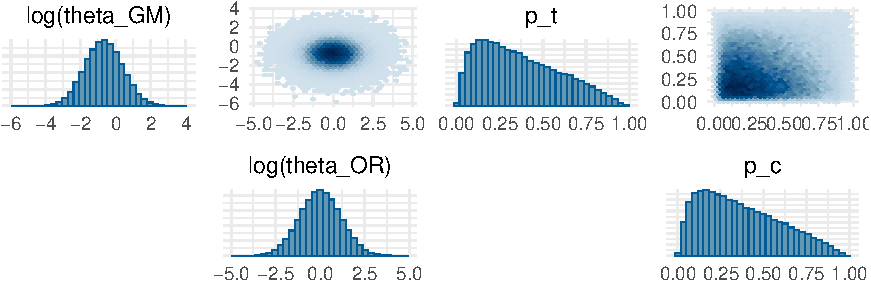
\includegraphics{binom_sampling_workflow_files/figure-beamer/binom_theta_priorpreds-1} \end{flushleft}

\end{frame}

\begin{frame}{Rethinking the Model}
\protect\hypertarget{rethinking-the-model-3}{}

What do our priors for \(\theta_{GM}\) and \(\theta_{OR}\) imply about
\(p_T,\ p_C\), and \(\mb{Y}\)? \vspace{-0.1in}

\begin{itemize}
\tightlist
\item
  Prior predictive distribution: (1) draw
  \(\wtil{\theta}_{GM}\sim \pi(\theta_{GM}),\ \wtil{\theta}_{OR}\sim\pi(\theta_{OR}) \implies(\wtil{p}_T,\wtil{p}_C)\),
  then (2) simulate outcomes
  \(\wtil{Y}_T\sim \mr{Binomial}(N_T,\wtil{p}_T),\ \text{and } \wtil{Y}_C\sim\mr{Binomial}(N_C,\wtil{p}_C).\)
\item
  Summary statistics of interest (90\% prior predictive interval): total
  deaths (8, 48) , deaths per arm (2, 29), absolute difference in deaths
  per arm (1, 24).
\end{itemize}

\begin{center}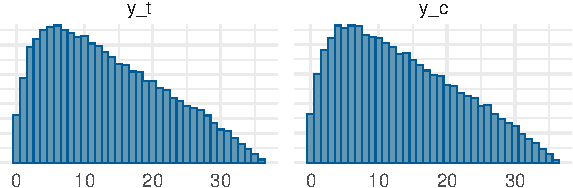
\includegraphics{binom_sampling_workflow_files/figure-beamer/binom_cases_priorpreds-1} \end{center}

\end{frame}

\begin{frame}{Rethinking the Model}
\protect\hypertarget{rethinking-the-model-4}{}

Suppose we had stuck with
\(p_T\sim \mr{Beta}(1,1),\ p_C\sim \mr{Beta}(1,1)\). What are the
induced priors on \(\theta_{GM},\ \theta_{OR}\), and \(\mb{Y}\)?

\begin{flushleft}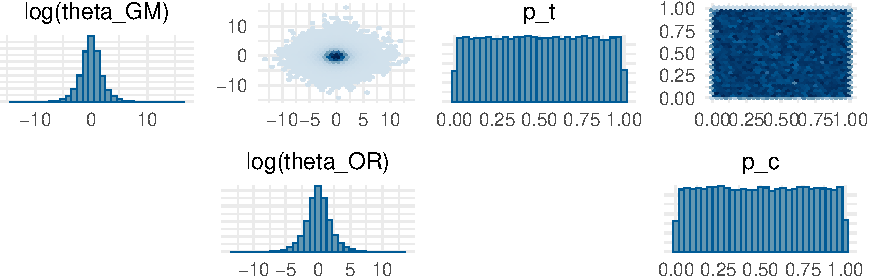
\includegraphics{binom_sampling_workflow_files/figure-beamer/binom_theta_priorpreds_unif-1} \end{flushleft}

\end{frame}

\begin{frame}{Rethinking the Model}
\protect\hypertarget{rethinking-the-model-5}{}

Suppose we had stuck with
\(p_T\sim \mr{Beta}(1,1),\ p_C\sim \mr{Beta}(1,1)\). What are the
induced priors on \(\theta_{GM},\ \theta_{OR}\), and \(\mb{Y}\)?

\begin{itemize}
\tightlist
\item
  Summary statistics of interest (90\% prior predictive interval): total
  deaths (11, 61) , deaths per arm (1, 35), absolute difference in
  deaths per arm (1, 29).
\end{itemize}

\begin{center}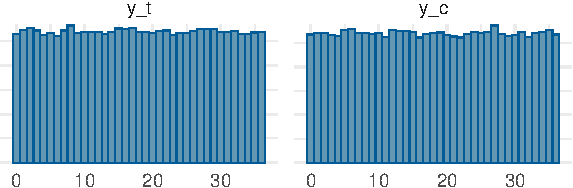
\includegraphics{binom_sampling_workflow_files/figure-beamer/binom_cases_priorpreds_unif-1} \end{center}

\end{frame}

\begin{frame}{MCMC for Non-conjugate Priors}
\protect\hypertarget{mcmc-for-non-conjugate-priors}{}

Posterior distribution no longer analytically available. Let's do that
MCMC!\vspace{-0.1in}

To specify the model in \texttt{Stan}, we need to define (at a
minimum)\vspace{-0.1in}

\begin{itemize}
\tightlist
\item
  \emph{Data}: \(\mb{N},\ \mb{Y}\),
\item
  \emph{Parameters}: \(\theta_{GM},\theta_{OR}\),
\item
  \emph{Model}: Binomial likelihood, log-normal priors.
\end{itemize}

Optionally, we can also specify\vspace{-0.1in}

\begin{itemize}
\tightlist
\item
  \emph{User-defined functions}: e.g., for manipulating data,
  transforming parameters,
\item
  \emph{Transformed data}: e.g., centered covariates,
\item
  \emph{Transformed parameters}: \(p_T,\ p_C\),
\item
  \emph{Generated quantities}: functionals of parameters, posterior
  predictive samples.
\end{itemize}

Each of these is defined in a block of \texttt{Stan} code, which is
compiled into \texttt{C++}.

\texttt{Stan} has incredible
\href{https://mc-stan.org/users/documentation/}{\textcolor{blue}{documentation}}
and an active (and very supportive)
\href{https://mc-stan.org/community/}{\textcolor{blue}{user community}}
that you can lean on if you ever need help with a model.

\end{frame}

\begin{frame}[fragile]{Let's do that MCMC!}
\protect\hypertarget{lets-do-that-mcmc}{}

\textbf{Data:} \vspace{-0.1in}

\begin{itemize}
\tightlist
\item
  The data, but also any quantities that are needed to instatiate
  objects, e.g., dimensions of matrices.
\item
  Objects here are fixed, no random variables declared here.
\end{itemize}

\begin{verbatim}
data {
  int<lower=0> N[2]; // sample sizes per arm
  int<lower=0> y[2]; // numbers of deaths per arm
}
\end{verbatim}

\end{frame}

\begin{frame}[fragile]{Let's do that MCMC!}
\protect\hypertarget{lets-do-that-mcmc-1}{}

\textbf{Parameters:} \vspace{-0.1in}

\begin{itemize}
\tightlist
\item
  Correspond to the variables being sampled in the MCMC.
\item
  Constraints for safety and to tell \texttt{Stan} how to transform to
  avoid boundaries of parameter space.
\item
  \texttt{Stan} defines an unnormalized log-probability over
  unconstrained parameters and adds Jacobians automatically.
\end{itemize}

\begin{verbatim}
parameters {
  real<lower=0> theta_GM; // geometric mean odds of death
  real<lower=0> theta_OR; // odds ratio
}
transformed parameters {
  real<lower=0,upper=1> probs[2]; 
  probs[1] = inv_logit(log(theta_GM) + 0.5 * log(theta_OR)); // p_T
  probs[2] = inv_logit(log(theta_GM) - 0.5 * log(theta_OR)); // p_C
}
\end{verbatim}

\end{frame}

\begin{frame}[fragile]{Let's do that MCMC!}
\protect\hypertarget{lets-do-that-mcmc-2}{}

\textbf{Model:} \vspace{-0.1in}

\begin{itemize}
\tightlist
\item
  Sampling statements define contributions to the log-posterior.
\item
  Includes both priors and likelihood.
\item
  If declare priors for transformed parameters, need to manually add a
  Jacobian adjustment.
\end{itemize}

\begin{verbatim}
model {
  y ~ binomial(N, probs);               // likelihood
  theta_GM ~ lognormal(log(0.5), 1.08); // prior for theta_GM
  theta_OR ~ lognormal(0, 1.08);        // prior for theta_OR
}
\end{verbatim}

\end{frame}

\begin{frame}[fragile]{Let's do that MCMC!}
\protect\hypertarget{lets-do-that-mcmc-3}{}

\textbf{Generated quantities:}

\begin{itemize}
\tightlist
\item
  Posterior predictives and derived quantities computed online and
  returned in MCMC output.
\item
  Later, compute log-likelihoods for model comparison.
\end{itemize}

\begin{verbatim}
generated quantities {
  int y_pp[2] = binomial_rng(N, probs); // simulate from posterior predictive
  real rr_pp = probs[1] / probs[2];     // relative risk
  real rd_pp = probs[1] - probs[2];     // risk difference
}
\end{verbatim}

\end{frame}

\begin{frame}[fragile]{Let's do that MCMC!}
\protect\hypertarget{lets-do-that-mcmc-4}{}

Running the model in R: \vspace{-0.1in}

\begin{itemize}
\tightlist
\item
  Write \texttt{Stan} code into a \texttt{.stan} file (RStudio: File
  \textgreater{} New File \textgreater{} Stan File).
\item
  Probably something similar in Python, I dunno.
\item
  Compile and run as follows:
\end{itemize}

\begin{Shaded}
\begin{Highlighting}[]
\NormalTok{prevailmod =}\StringTok{ }\KeywordTok{stan_model}\NormalTok{(}\DataTypeTok{file =} \StringTok{"prevailmod.stan"}\NormalTok{) }\CommentTok{# compile model}
\NormalTok{data =}\StringTok{ }\KeywordTok{list}\NormalTok{(}\DataTypeTok{N =} \KeywordTok{c}\NormalTok{(}\DataTypeTok{ZMapp =} \DecValTok{36}\NormalTok{, }\DataTypeTok{oSOC =} \DecValTok{35}\NormalTok{),         }\CommentTok{# numbers of participants}
            \DataTypeTok{y =} \KeywordTok{c}\NormalTok{(}\DataTypeTok{ZMapp =} \DecValTok{8}\NormalTok{, }\DataTypeTok{oSOC =} \DecValTok{13}\NormalTok{))          }\CommentTok{# deaths per arm}
\NormalTok{prevailfit =}\StringTok{ }\KeywordTok{sampling}\NormalTok{(}\DataTypeTok{object =}\NormalTok{ prevailmod,        }\CommentTok{# compiled model}
                      \DataTypeTok{data   =}\NormalTok{ data,              }\CommentTok{# data}
                      \DataTypeTok{chains =} \DecValTok{5}\NormalTok{,                 }\CommentTok{# number of chains (>1 !!!!)}
                      \DataTypeTok{iter   =} \FloatTok{2e3}\NormalTok{)               }\CommentTok{# number of iterations}
\end{Highlighting}
\end{Shaded}

\end{frame}

\begin{frame}{MCMC Output}
\protect\hypertarget{mcmc-output}{}

\texttt{Stan} produces correlated MCMC samples from the posterior via
Hamiltonian Monte Carlo.

\begin{center}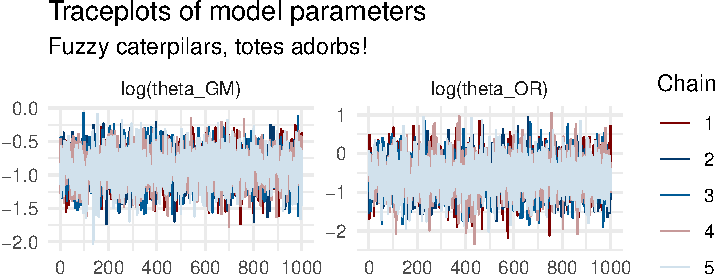
\includegraphics{binom_sampling_workflow_files/figure-beamer/stan_traces-1} \end{center}

\end{frame}

\begin{frame}[fragile]{MCMC Diagnostics}
\protect\hypertarget{mcmc-diagnostics}{}

Lots of diagnostics,
\href{http://mc-stan.org/misc/warnings.html}{\textcolor{blue}{always check your diagnostics}}.
More
\href{https://mc-stan.org/rstan/reference/stan_plot_diagnostics.html}{\textcolor{blue}{here}}
and in the \texttt{Stan} reference manual.

\begin{verbatim}
##      accept_stat__ stepsize__ treedepth__ n_leapfrog__ divergent__
## [1,]     1.0000000  0.9754109           2            3           0
## [2,]     0.7390574  0.9754109           2            3           0
## [3,]     1.0000000  0.9754109           2            3           0
## [4,]     0.9621533  0.9754109           1            3           0
## [5,]     0.8248869  0.9754109           2            3           0
##      energy__
## [1,] 44.60989
## [2,] 45.24771
## [3,] 45.31665
## [4,] 45.22013
## [5,] 43.54042
\end{verbatim}

\end{frame}

\begin{frame}[fragile]{Results}
\protect\hypertarget{results}{}

Marginal summaries\footnote<.->{In Beta-Binomial model with Uniform(0,1)
  priors:
  \(p_T = 0.23 (0.12, 0.38);\ p_C = 0.38 (0.23, 0.54);\ RD = -0.14 (-0.34, 0.06); RR = 0.62 (0.29, 1.24); OR = 0.50(0.18, 1.36).\)}:\vspace{-0.15in}

\begin{verbatim}
##                mean     se_mean         sd       2.5%        25%
## theta_GM  0.4213551 0.001759412 0.10718448  0.2417749  0.3456898
## theta_OR  0.6241425 0.005282141 0.30981109  0.2282034  0.4083772
## probs[1]  0.2399010 0.001075035 0.06349585  0.1278092  0.1946408
## probs[2]  0.3564025 0.001106634 0.07330828  0.2184726  0.3047550
## rr_pp     0.7012247 0.004023744 0.23996935  0.3424526  0.5311668
## rd_pp    -0.1165015 0.001434496 0.09249205 -0.2934280 -0.1799115
##                 50%         75%      97.5%    n_eff      Rhat
## theta_GM  0.4092737  0.48563778 0.66043117 3711.323 1.0004128
## theta_OR  0.5584364  0.76411135 1.39572402 3440.123 0.9999599
## probs[1]  0.2355453  0.28230435 0.37421211 3488.555 0.9998798
## probs[2]  0.3548359  0.40579766 0.49962301 4388.314 1.0004480
## rr_pp     0.6647296  0.82959835 1.27363815 3556.729 0.9998410
## rd_pp    -0.1188121 -0.05450594 0.06559438 4157.287 0.9998778
\end{verbatim}

\end{frame}

\begin{frame}{Results}
\protect\hypertarget{results-1}{}

Posterior distributions of model parameters.

\begin{center}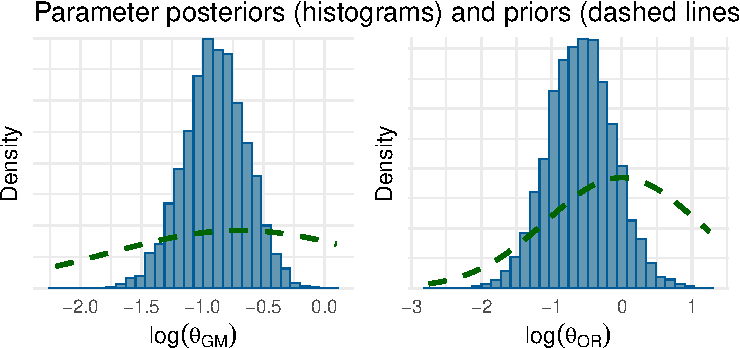
\includegraphics{binom_sampling_workflow_files/figure-beamer/prevail_posts-1} \end{center}

\end{frame}

\begin{frame}{Results}
\protect\hypertarget{results-2}{}

Can do better than marginal summaries, we have access to the
\emph{joint} posterior!

\begin{center}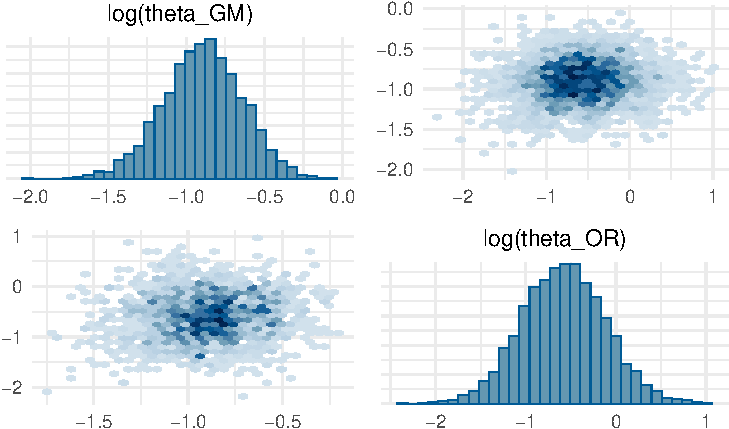
\includegraphics{binom_sampling_workflow_files/figure-beamer/prevail_pairs-1} \end{center}

\end{frame}

\begin{frame}{Posterior Predictive Distribution}
\protect\hypertarget{posterior-predictive-distribution}{}

We can sample from the posterior predictive distribution by iteratively
drawing \(\wtil{\theta}_{post}\sim \pi(\theta|y)\), then simulating
\(\wtil{Y}|\wtil{\theta}_{post} \sim \mr{Binomial}(N,\wtil{p}_{post}).\)

Suppose we want to predict 28 day mortality for 10 new individuals in
each group.

\begin{center}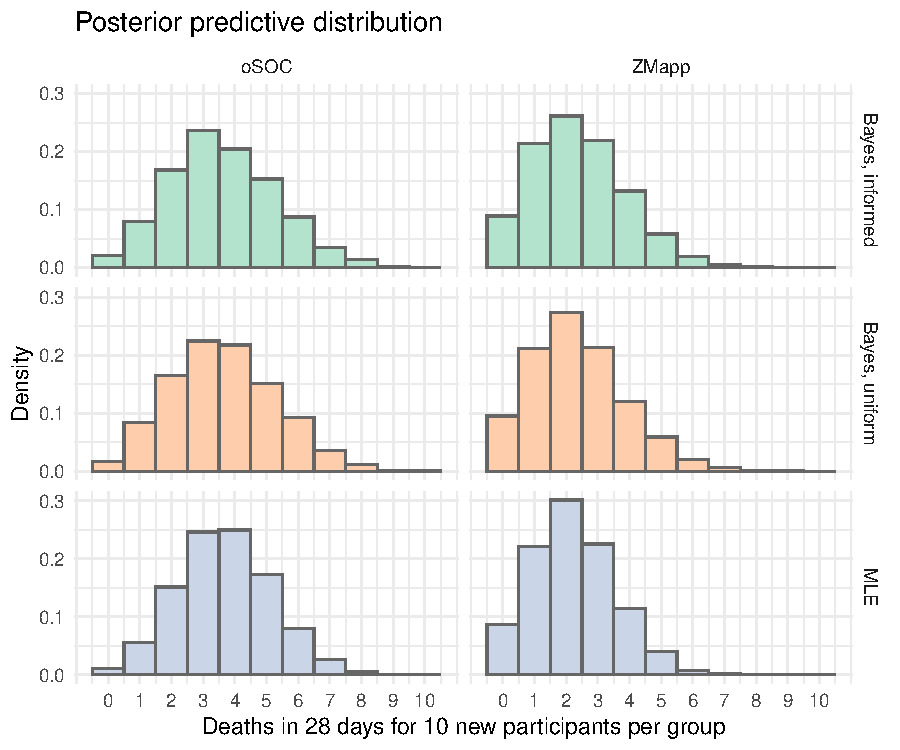
\includegraphics[width=0.5\linewidth]{predplot} \end{center}

\end{frame}

\begin{frame}{Next time}
\protect\hypertarget{next-time}{}

No meeting next week (Labor Day). In two weeks we'll talk about linear
regression (for real this time).

\begin{itemize}
\tightlist
\item
  Setting weakly (not weekly) informative priors.
\item
  Assessing failure modes of different priors.
\item
  More Stan.
\end{itemize}

Watch/rewatch lecture 3 and first half of 4 (SmaRt).

\end{frame}

\begin{frame}{References}
\protect\hypertarget{references}{}

M. Betancourt ``Calibrating model-based inferences and decisions.''
arXiv preprint arXiv:1803.08393 (2018).

M. Betancourt ``Toward a principled Bayesian workflow.''
\url{https://betanalpha.github.io/assets/case_studies/principled_bayesian_workflow.html}
(2018).

J. Gabry, et al. ``Visualization in Bayesian workflow.'' \emph{Journal
of the Royal Statistical Society: Series A (Statistics in Society)}
182.2 (2019): 389-402.

\end{frame}

\begin{frame}{}
\protect\hypertarget{section}{}

\end{frame}

\end{document}